% !TeX root = Dokumentation.tex

\section{Neo4J}
Neo4J ist eine in Java implementierte Graphdatenbank, die sich gut dazu eignet um unstrukturierte Daten zu speichern und zu verwalten.

\vspace{6pt}

Im Rahmen des Moduls Moderne Datenbanken haben wir Gruppenaufgaben zu Neo4J bekommen. Für diese werden die Lösungsideen und Aspekte dieser betrachtet und beschrieben. 

\vspace{18pt} 

\subsection{Aufgabenstellung}
Jeder Gruppe wurden für Neo4J sechs Aufgaben gegeben. Diese sind den Folien zu entnehmen. Besagte Aufgaben wurden von Prof. Königsmann genauer spezifiziert und abgeändert. Wir haben die Aufgaben wie folgend verstanden:

\begin{enumerate}
	\item Unsere Datenbank soll auf Neo4J umgestellt werden. Dabei sollen in Neo4J die gleichen Informationen abrufbar sein, wie vorher.
	\item Wir sollen mindestens drei sinnvolle Erweiterungen für unser Datenbank-Schema identifizieren. Diese zu implementieren ist nicht vorgesehen.
	\item Es müssen Daten persistiert werden.
	\item Es soll die Performance von Create, Read, Update und Delete-Operationen getestet werden.
	\item Die existierenden Relationalen-abfragen für die Datenbank sollen in Neo4J abgebildet werden.
	\item Wir sollen mindestens drei Beispiele finden, in denen sich Neo4J besonders gut eignet.
\end{enumerate}

\subsection{Datenbankschema} 
Das aktuelle Datenbankschema und die Tabellen sind dem folgenden Bild zu entnehmen.
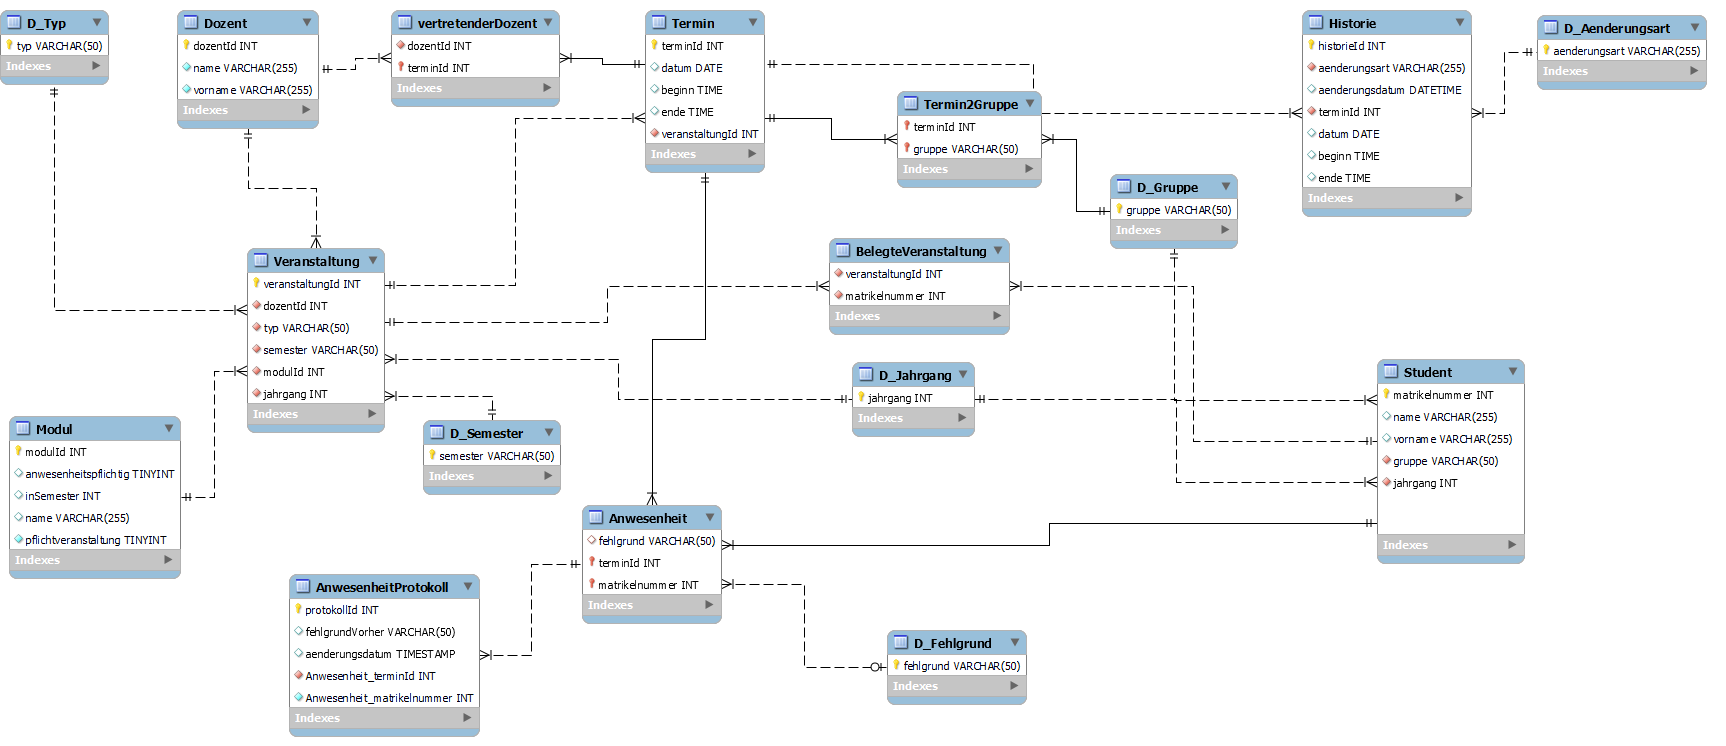
\includegraphics[width=\textwidth]{studenplanDBmodel.png}
Die Tabellen des jetzigen Datenbankschemas lassen sich in die drei Kategorien \textbf{Entity}, \textbf{Relation} und \textbf{Domain} unterteilen.

\vspace{12pt}

\subsubsection{Entity}
Eine Tabelle, die Fachliche Objekte bzw. Informationen Enthält, kann und wird in Neo4J durch Knoten dargestellt. Also wird jedes Tupel aus einer Entitäts-Tabelle zu einem Label. Die folgenden Tabellen wurden dieser Kategorie zugeteilt.
17
\begin{itemize}
	\item Dozent
	\item Termin
	\item Veranstaltung
	\item Modul
	\item Student
	\item Historie (Wird nicht weiter betrachtet, weil sich unserer Meinung nach neo4J schlecht dafür eignet eine Historie von Änderungen darzustellen)
\end{itemize}

\vspace{12pt}

\subsubsection{Releation}
Relationstabellen sind Matching Tabellen. Diese werden sich in Beziehungen zwischen den knoten auflösen. Die folgenden Tabellen wurden dieser Kategorie zugeteilt.

\begin{itemize}
	\item vertretenderDozent
	\item Termin2Gruppe (Wird nicht weiter mit einbezogen, weil diese Tabelle keine Rolle für Funktionsfähigkeit des Projektes spielt.)
	\item BelegteVeranstaltung
	\item Anwesenheit
\end{itemize}

\vspace{12pt}

\subsubsection{Domain}
Eine Domain Tabelle ist eine Tabelle, die in einer Relationalen Datenbank für die Konsistenz von Daten sorgt. So eine Tabelle besteht häufig nur aus einer Spalte. Dadurch soll sichergestellt werden, dass nur vordefinierte Werde benutzt werden können. Diese Tabellen werden beider Konvertierung zu Neo4J wegfallen. Die folgenden Tabellen wurden dieser Kategorie zugeteilt.

\begin{itemize}
	\item D\_Typ
	\item D\_Gruppe
	\item D\_Aenderungsart
	\item D\_Semester
	\item D\_Jahrgang
	\item D\_Fehlgrund	
\end{itemize}

\vspace{12pt}

\subsubsection{Ergebnis}
Wir haben die folgenden Labels und Beziehungen ausgearbeitet.

\vspace{6pt}

\paragraph{Labels}
\begin{itemize}
	\item Dozent
	\item Termin
	\item Modul
	\item Veranstaltung
	\item Student
\end{itemize}

\vspace{6pt}

\paragraph{Beziehungen}
\begin{itemize}
	\item VERTRITT\_IN
	\item BELEGT\_VERANSTALTUNG
	\item NICHT\_ANWESEND
	\item HAT
\end{itemize}

\newpage

\subsection{Erweiterungen}
Wir sollen drei sinnvolle Erweiterungen ausarbeiten. Einmal soll nachvollziehbar sein, welche Module aufeinander aufbauen. Zum anderen sollen Studenten, die das Modul gerade machen, Studenten finden können, die das Modul bereits abgeschlossen haben und um Hilfe bitten. 

\vspace{12pt}

\subsubsection{Aufeinander aufbauende Module}
Es gibt Module, die aufeinander aufbauen. Das wird im Jetzigen Zustand nicht von unserem Datenbankschema abgebildet. Es gibt bereits Modul-Knoten. Hier wird nur eine weitere Beziehung hinzugefügt, die \textbf{BASIERT\_AUF} heißt und darstellt, dass in dem Modul davon ausgegangen wird, dass andere Module bereits absolviert wurden.

\vspace{12pt}

\subsubsection{Vertiefungen}
Es gibt Vertiefungen. Eine Vertiefung ist eine Gruppierung von Modulen, die Logisch zusammen gehören und einzelne Themen eines Großen Themas behandeln. Im Augenblick gibt es keine Möglichkeit, die Gruppierung von Modulen darzustellen. Dafür muss ein neuer Knotentyp und eine neue Beziehung hinzugefügt werden. Der Knotentyp heißt \textbf{Vertiefung}. Die neue Beziehung heißt \textbf{BESTEHT\_AUS}. Eine Vertiefung hat einen Namen.

\vspace{12pt}

\subsubsection{Hilfe unter Studenten}
Zum anderen sollen Studenten, die das Modul gerade machen, Studenten finden können, die das Modul bereits abgeschlossen haben und um Hilfe bitten.

\newpage

\subsection{Daten}
Nachdem bestimmt wurde, wie die Daten gespeichert werden, sollen sinnvolle Daten gespeichert werden.
